\appendixchapter{Track reconstruction in the CMS FastSimulation package}
\label{ch:fsim}

\intro{Simulated samples of events are a key ingredient within analyses for understanding the detector and the physics behind \gls{lhc} collision data. An introduction to the FastSimulation (\gls{fsim}) package of \gls{cms} is given in this chapter. It provides a fast alternative for simulating the detector response and emulating the reconstruction of events compared to the standard simulation and reconstruction workflow of \gls{cms}. This is achieved by replacing some computing-intense parts in the standard simulation and reconstruction chain with various approximations. One particular speedup is obtained by using an own track reconstruction which relies on truth information to solve the combinatorial problem of associating reconstructed hits to trajectories. In addition, details about the generation of reconstructed hits in the inner tracking system and the seeding of trajectory in \gls{fsim} are given. Before the chapter is concluded the performance of the emulated track reconstruction is validated. This chapter is mostly based on Ref.~\cite{fastsim-mkomm}.}

\todo{update ref when proceedings accepted}


%##############################################
\section{Introduction}
%##############################################

Simulating the detector response for arbitrary events is of crucial importance for understanding recorded collision data and to infer properties of the underlying physics in analyses. The standard package for simulation collision events in \gls{cms} is called ``FullSimulation''~\cite{1742-6596-396-2-022003,1742-6596-664-7-072022}. It is based on the \GEANT{}4 toolkit~\cite{Agostinelli2003250} and provides a detailed simulation of the detector response and an emulation of its readout systems. Simulated events are reconstructed utilizing the same event reconstruction algorithms as utilized for data.

A fast alternative to the standard simulation and reconstruction workflow is provided by the ``FastSimulation'' (\FSIM[format=hyperbf]) package of \gls{cms}. It delivers high-level analysis objects with sufficient accuracy for analyses while being tightly integrated into the \gls{cms} software framework~\cite{Bayatian:922757} along the standard simulation and reconstruction workflow. Its simulation speed of less than 10~s per event\footnote{For events with up to $\approx30$ pileup interactions on average.} is achieved by sidestepping certain parts in the standard simulation and reconstruction chain and utilizing various approximations instead. The two major CPU-intense parts which are replaced are the \GEANT{}4-based~\cite{Agostinelli2003250} simulation of particle interactions with the detector material and the track reconstruction. In particular, the complex, multistep algorithms which reconstruct tracks from energy depositions left by traversing charged particles in the \gls{cms} inner tracking system are exchanged with simpler versions that rely on truth-information about the simulated events. The final analysis objects produced by \FSIM are indistinguishable from the ones produced by the standard simulation and reconstruction workflow. This enables an easy integration of \FSIM samples in analyses along standard simulation and data samples.

Nowadays, the \FSIM package is successfully employed within \gls{cms} analyses. Typical use cases are searches for \acrfull{bsm} physics like \acrfull{susy}. These analyses require usually multiple signal samples which reflect various realizations of a new physics model. Other use cases are the evaluation of the impact of systematic uncertainties on a measurement like a variation of the renormalization and factorization scales or the top quark mass. A more general use case is to increase the statistics of existing samples for training \acrfull{mva} methods. The development of \FSIM is further motivated in the light of increasing luminosity and data statistics for which larger samples of simulated events with higher pileup conditions have to be produced for analysis.

In this chapter the \FSIM package is introduced with an emphasis on the employed track reconstruction for simulated events as follows. First an overview of the standard simulation and the specialized \FSIM workflows are given in Sec.~\ref{sec:fsim-workflow}. Then, the generation of reconstructed hits (Sec.~\ref{sec:fsim-hits}) and the emulation of the iterative track reconstruction are detailed (Sec.~\ref{sec:fsim-tracking}) where the latter focuses in particular on the seeding of trajectories for initiating the iterative tracking sequence. A validation of the track reconstruction is presented in Sec.~\ref{sec:fsim-validation} where the obtain performances are compared with the result of the standard simulation and reconstruction. The chapter is concluded in Sec.~\ref{sec:fsim-conclusion}.


%##############################################
\section{Simulation workflow}
%##############################################
\label{sec:fsim-workflow}

The individual steps within the \gls{cms} software to obtain simulated events for comparison with data are sketched in the following with an emphasis on the differences between the standard and \FSIM workflows.

\begin{description}
\item[Generation] The sample generation commences by creating collections of particles with the help of \acrfull{mc} generators that are configured to produce events according to some physics process of interest. This step can also be performed independently of the core \gls{cms} software. Common interfaces with generator programs are provided through the \HEPMC[format=hyperbf]~\cite{Dobbs:2001ck} or \LHEF[format=hyperbf]~\cite{Alwall:2006yp} event formats.

\item[Simulation] The trajectories of the generated particles are propagated through a geometrical model of the detector starting from the interaction point. As the particles traverse the detector, their interaction with the encountered material is simulated. In the standard simulation, the \GEANT{}4 package is utilized which provides a detailed propagation of particles in the magnetic field and a sophisticated simulation of the various interactions. 
In \FSIM a simplified detector geometry is utilized for the inner tracking system. Interactions are only simulated on infinitely thin cylindrical layers and endcap disks using parameterized models for energy loss through ionization, bremsstrahlung, photon conversion, and multiple scattering. Since a constant magnetic field is assumed as well the propagation of particles between the layers is performed analytically. In a final step the intersection points of the trajectories with the simplified geometry are projected onto the real geometry of the tracking system to create simulated hits associated to actual tracker modules. In the calorimetry systems \gls{em} or hadronic showers are simulated by sampling energy deposits from parameterized models of the expected longitudinal and transverse shower profiles per particle type and energy.

\item[Digitalization] An emulation of the detector readout systems is performed in the digitalization step. After this stage, the event record in the standard simulation contains similar information as found in recorded raw data events. In \FSIM the digitalization algorithms of the standard simulation workflow are also utilized for the calorimeter systems. For the tracker hits no detailed simulation of the charge deposition is performed. Instead, the reconstruction of hits from charge clusters is only emulated by performing a smearing of the simulated hit positions are detailed in Sec.~\ref{sec:fsim-hits} below.

\item[Reconstruction] In \FSIM the standard event reconstruction is applied to simulated events as well with the exception of the track reconstruction. Here, the computing-intense tracking algorithm with includes amongst others the \acrfull{ctf} algorithm~\cite{Chatrchyan:2014fea} are bypassed by utilizing truth-information about the simulated events instead to solve the combinatorial problem.
\end{description}

The tight integration of the \FSIM package within the \gls{cms} software allows to utilize most of the standard data containers within its workflow so that simulated \FSIM samples can easily be used by analysts along samples generated with the standard event simulation and reconstructed data. 


%##############################################
\section{Emulation of hit reconstruction}
%##############################################
\label{sec:fsim-hits}

An emulation of the local hit reconstruction for the tracker modules has to be performed since no detailed information of charge deposition is generated in the simulation step of \FSIM. To mimic the resolutions of the standard hit reconstruction the true hit positions are smeared. A new \FSIM module for position smearing has been developed which allows to manage various algorithms for position smearing side-by-side. It can be flexibly configured for any topology of the tracker. Additionally, each algorithm can be restricted to certain tracker modules only. A sketch of the inner workings of the new module is shown in Fig.~\ref{fig:fsim-hitsmearing}.

\myfigure{\label{fig:fsim-hitsmearing}Emulation of local hit reconstruction in \FSIM.  Various algorithm can be configured side-by-side. A flexible selection syntax allows to specify on a per module basis which hits to process.}{
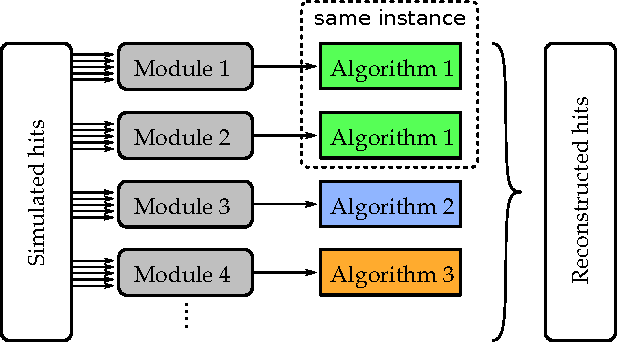
\includegraphics[scale=0.75]{figures/fastsim/parcels.pdf}
}

First, the simulated hits are sorted according the associated tracker module. Then, algorithms for hit position smearing are loaded dynamically based on a configuration that is supplied by the user. Each instance of an algorithm can be configured to select and process only hits belonging to certain tracker modules. The selection is achieved through a special syntax parser for evaluating the user configuration dynamically against the module properties. Technically, the \texttt{Boost.Spirit} framework~\cite{boostspirit} is utilized to implement the parser based on grammar rules written in \glshere{ebnf}~\cite{ebnf}. This allows to extended the syntax easily in case of future requirements that are at the moment uncovered.

Currently, a simple Gaussian smearing of the position is employed for all strip modules where the configured resolution depends on the specific tracker subdetector (\gls{tib}, \gls{tid}, \gls{tob}, \gls{tec}) and its layer. A more detailed emulation of hit reconstruction is performed for the pixel modules where parametrized distributions from the standard template-based hit reconstruction are utilized for the smearing. These templates are generated using the \texttt{PixelAV} program which simulates the distributions of charges in pixel modules while accounting for their Lorentz drift in the magnetic field and potential radiation damage of the sensor~\cite{Swartz:2002kda}. The new \FSIM module allows furthermore the emulation of producing merged hits which occur in data when the distributions of the deposited charges from two particles transversing a tracker module overlap. Figure~\ref{fig:fsim-merge} shows a recent study of the probability of hit merging on the pixel modules. Such probability maps are expected to be used for the emulation of hit merging in the future.


\myfigure{\label{fig:fsim-merge}Probability of two hits merging on the pixel barrel modules as a function of their distance and local incident angle of a track expressed in pseudorapidity.}{
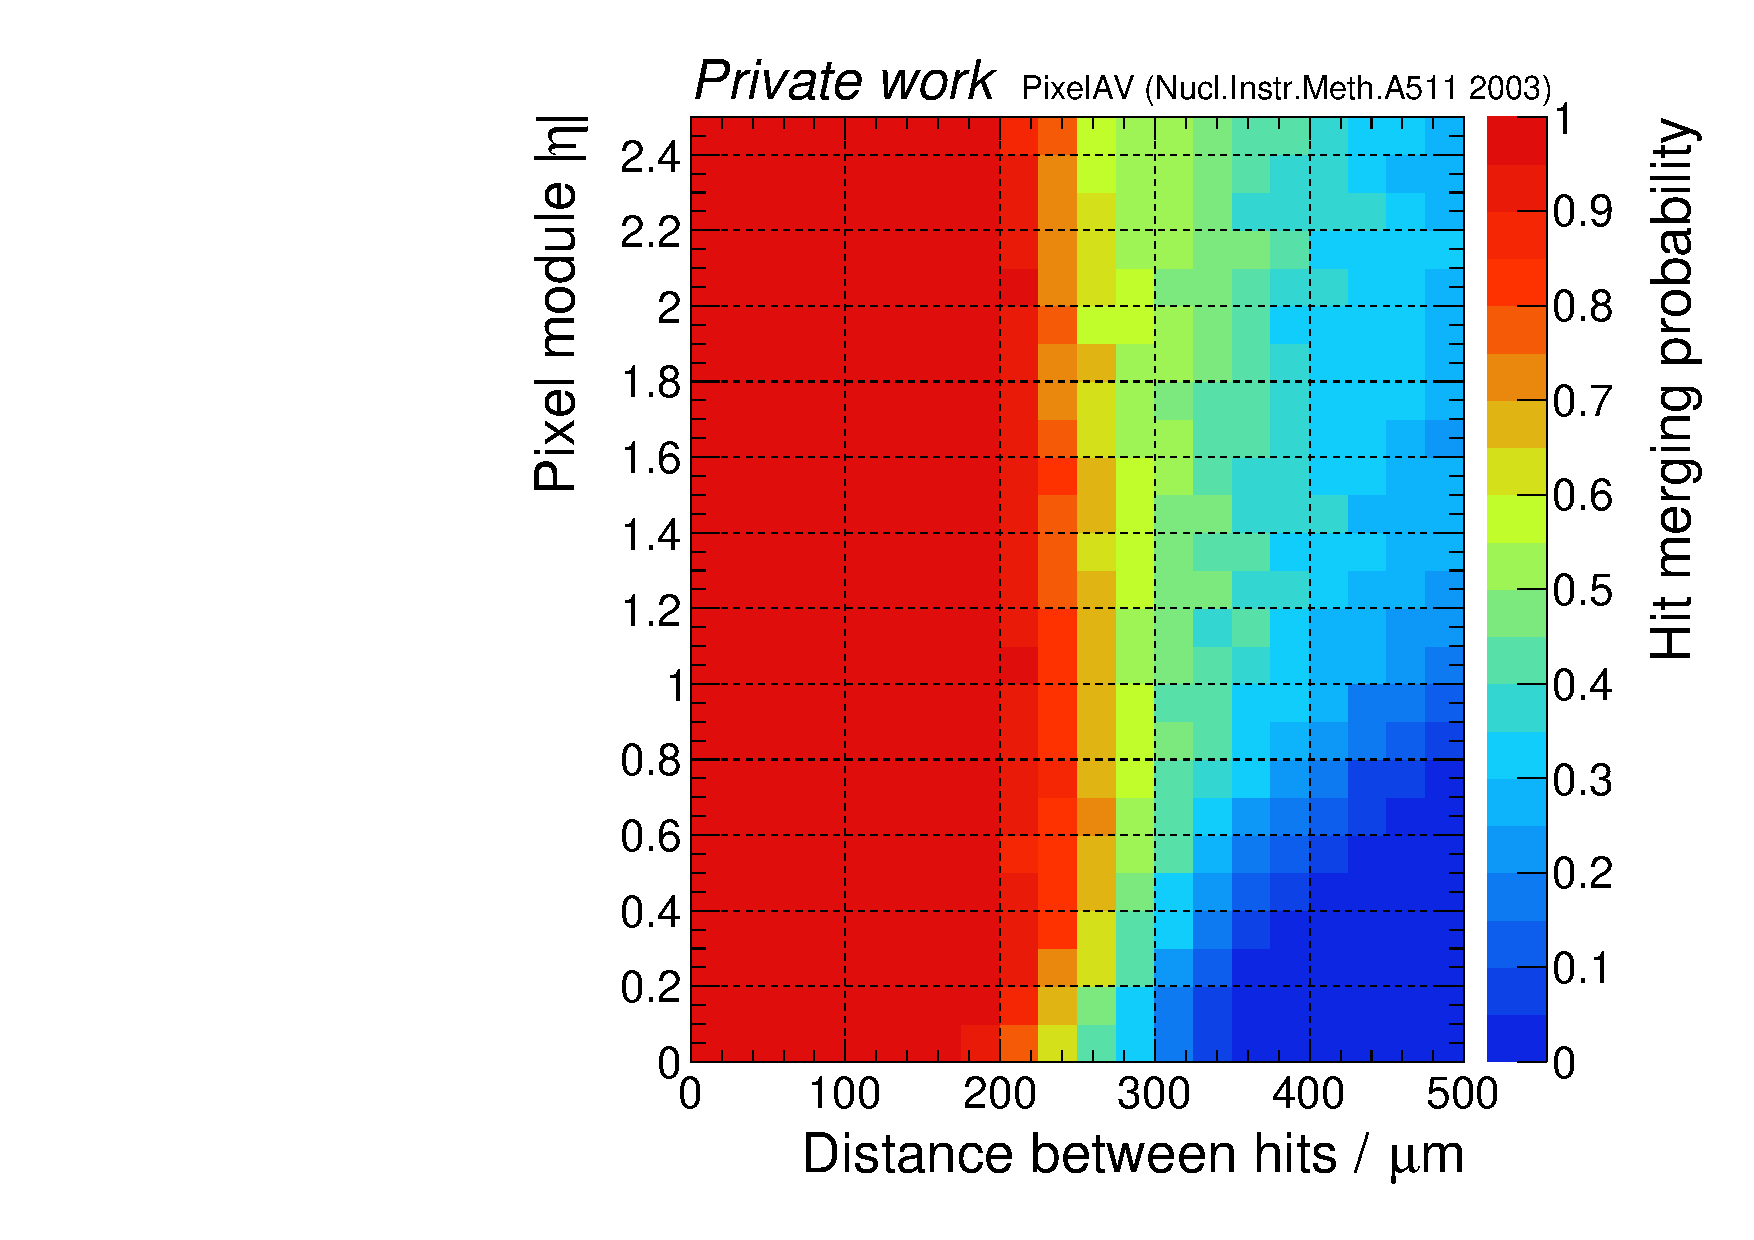
\includegraphics[width=0.48\textwidth]{figures/fastsim/merge.pdf}
}




%##############################################
\section{Emulation of track reconstruction}
%##############################################
\label{sec:fsim-tracking}

In \FSIM an emulation of the iterative track reconstruction is performed. The sequence of seeding, trajectory building and fitting and the iterative steps are kept similar to the standard track reconstruction but all algorithms are replaced with \FSIM-specific versions. A central idea to speedup the track reconstruction in \FSIM is to solve the combinatorial problem of associating reconstructed hits to particle trajectories by using \gls{mc}-truth information. An overview of the idea is shown in Fig.~\ref{fig:fsim-tracking}. Starting from a collection containing all reconstructed hits, each hit is mapped back to the simulated track from which it originated in the simulation. Then, the iterative tracking is carried out where each step is performed multiple times per subset of hits that belong to a single simulated track. This approach circumvents entirely any combinatorial confusion of hits. Thus, no fake tracks from a combination of spurious hits are emulated and the resulting tracking efficiency would in principle be 100\%. However, by accounting for dedicated selection criteria that are specified for each iteration in the standard reconstruction, the efficiency is decreased and becomes comparable to the one obtained in the standard track reconstruction as demonstrated in Sec.~\ref{sec:fsim-validation} below.

\myfigure{\label{fig:fsim-tracking}The track reconstruction workflow in \FSIM. Details are given in the text.}{
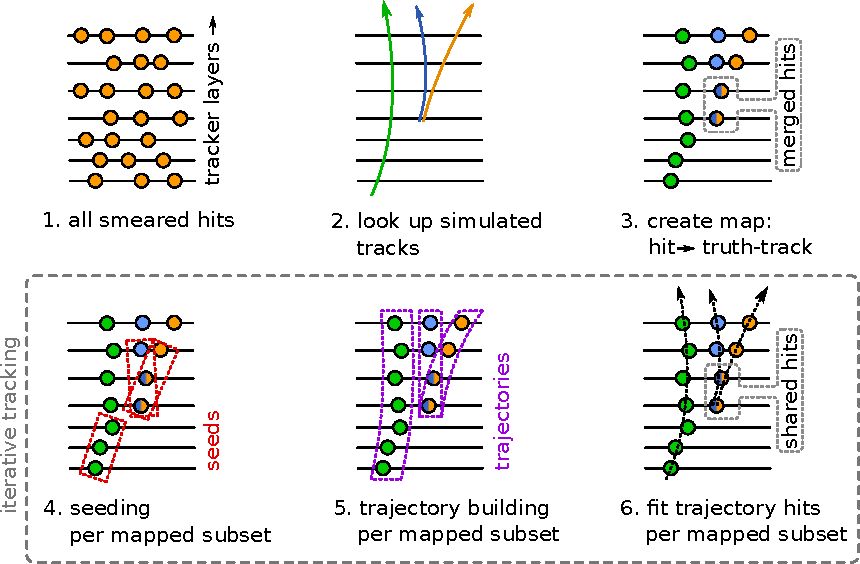
\includegraphics[scale=0.75]{figures/fastsim/tracking.pdf}
}

The ability to produce merged hits originating from close particle tracks necessitated a recent extension of the \FSIM{}-specific data containers within the iterative tracking sequence. Instead of a one-to-one mapping of reconstructed hits to simulated tracks, close simulated hits can now result into a single reconstructed ``merged'' hit that can be shared between the final tracks within an iteration as indicated in Fig.~\ref{fig:fsim-tracking}. A further benefit of the extension is that the mapping itself can be generated independently from the simulated track information which will allow the mix-in of wrong hit combinations leading to ``fake'' tracks in the future which is currently not emulated.


%##############################################
\subsection{New seeding algorithm}
%##############################################
\label{sec:fsim-seeding}

An algorithm has been developed to identify potential trajectory seed candidates while operating on an arbitrary number of seeding layers efficiently. In the original implementation, only doublets or triplets of hits could act as seeds. However, after the upgrade of the \gls{cms} pixel detector~\cite{Dominguez:1481838} a mixture of doublets, triplets, and quartets are utilized for seeding. This is solved in \FSIM by organizing the seeding layer configuration into a tree-like structure. For example the triplet configurations listed in Tab.~\ref{tab:fsim-seedinglist} can be transformed into the tree-structure as shown in Fig.~\ref{fig:fsim-seedingtree}. The new algorithm commences by iterating over a list of hits and linking them to a corresponding node in the tree. While the tree is being populated, dedicated seed selection criteria are evaluated on already found subsets of hits by interfacing directly with the standard track reconstruction. The exact selection is iteration-dependent and consists of various criteria such as the compatibility of the extrapolated trajectory with the beam spot or primary vertices\footnote{Preliminary primary vertices are reconstructed from tracks found in previous iterations.}. If hits at each node between the root and one of the leafs are found that are also compatible with any corresponding selection criteria the algorithm is stopped and the found seed candidate passed to the subsequent trajectory building and fitting stages as shown in Fig.~\ref{fig:fsim-tracking}.

\mytable{\label{tab:fsim-seedinglist}Exemplary configurations of pixel barrel (\gls{bpx}) and pixel forward (\gls{fpx}) layers where trajectory seed candidates can be generated from hits.}{
\begin{tabular}{@{}l l@{\,}l l@{\,}l l@{\,}l l@{\,}l l@{\,}l@{}}
\toprule
 & \multicolumn{10}{c}{Triplet layers} \\
First hit & BPX&1 & BPX&1 & BPX&1 & BPX&1 & BPX&1 \\
Second hit & BPX&2 & BPX&2 & BPX&2 & FPX+&1 & FPX-&1 \\
Third hit & BPX&3 & FPX+&1 & FPX-&1 & FPX+&2 & FPX-&2 \\
\bottomrule
\end{tabular}
}

\myfigure{\label{fig:fsim-seedingtree}Exemplary configurations of pixel barrel (\gls{bpx}) and pixel forward (\gls{fpx}) layers where trajectory seed candidates can be generated from hits. A seed has to contain corresponding hits at each node between the root and one of the leafs.}{
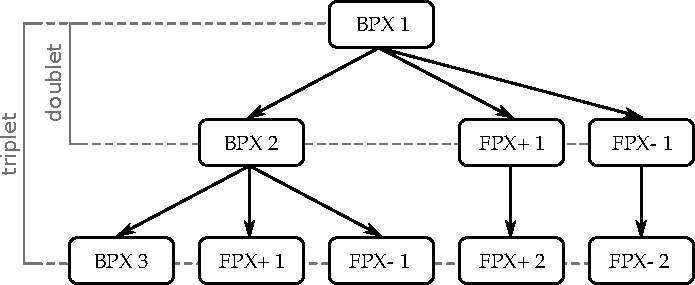
\includegraphics[scale=0.75]{figures/fastsim/seedingtree.pdf}
}

The developed tree-structure allows to performed seed generation from an arbitrary number of layers without using nested or recursive iterations over the reconstructed hits which makes it also fairly efficient.

%##############################################
\section{Validation}
%##############################################
\label{sec:fsim-validation}

The track reconstruction within \FSIM is validated by comparing the produced tracks with those obtained from the standard simulation and reconstruction workflow. A comparison of the resulting tracking efficiency as a function of the transverse momentum and pseudorapidity is presented in Fig.~\ref{fig:fsim-eff-tracks}, where the tracking efficiency is defined as the ratio of reconstructed tracks matched to simulated charged particles over the total number of charged particles within the tracker volume. Furthermore, the obtained resolution of the transverse momentum for reconstructed tracks is shown in Fig.~\ref{fig:fsim-res-track}. Overall, the distributions demonstrate a good agreement of the \FSIM tracking performance with the one obtained from the standard simulation and reconstruction workflow.

\myfigure{\label{fig:fsim-eff-tracks}Comparison of the reconstruction efficiencies of tracks as a function of (a)~the transverse momentum and (b)~the pseudorapidity measured in the simulation of top quark pair production at 13~TeV.}{
\subfloat[]{\centering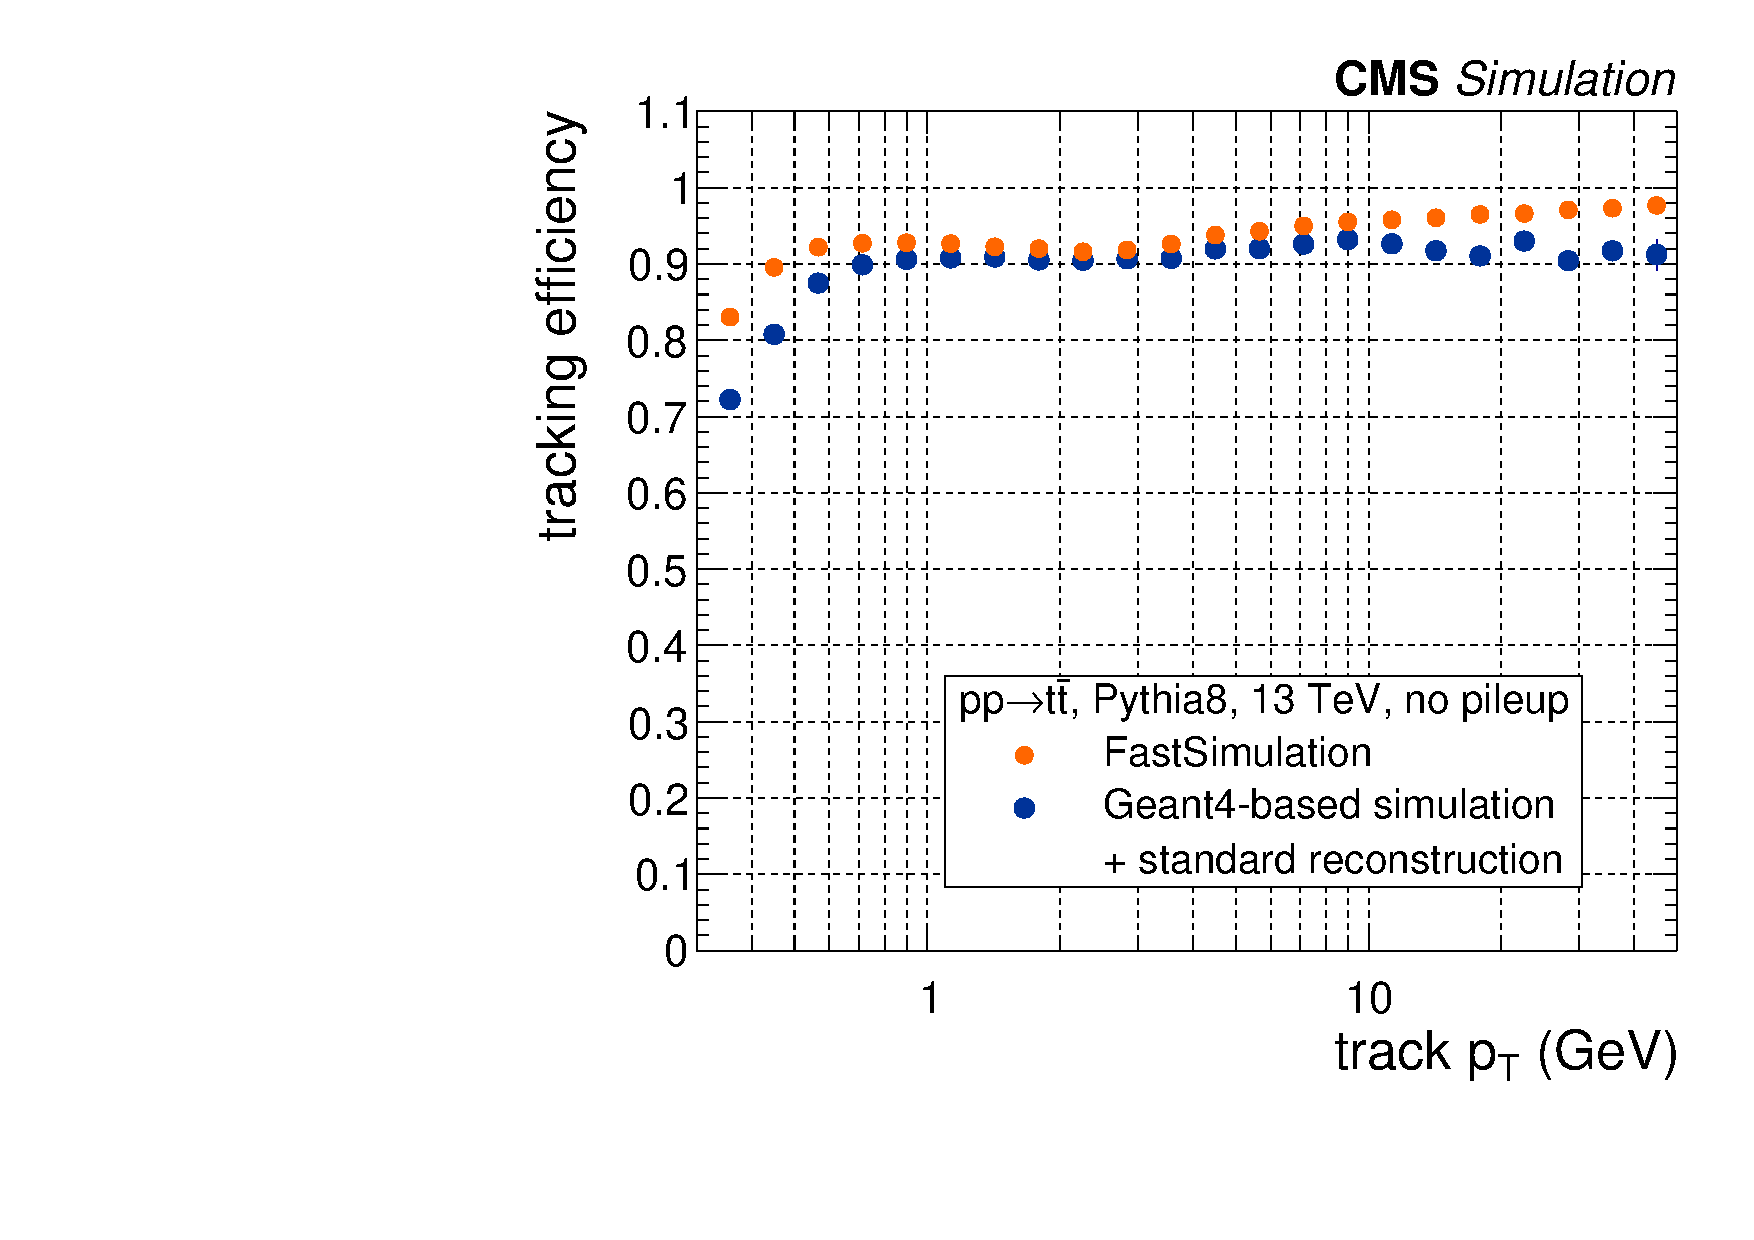
\includegraphics[width=0.48\textwidth]{figures/fastsim/eff_pt.pdf}}
\hspace{0.02\textwidth}
\subfloat[]{\centering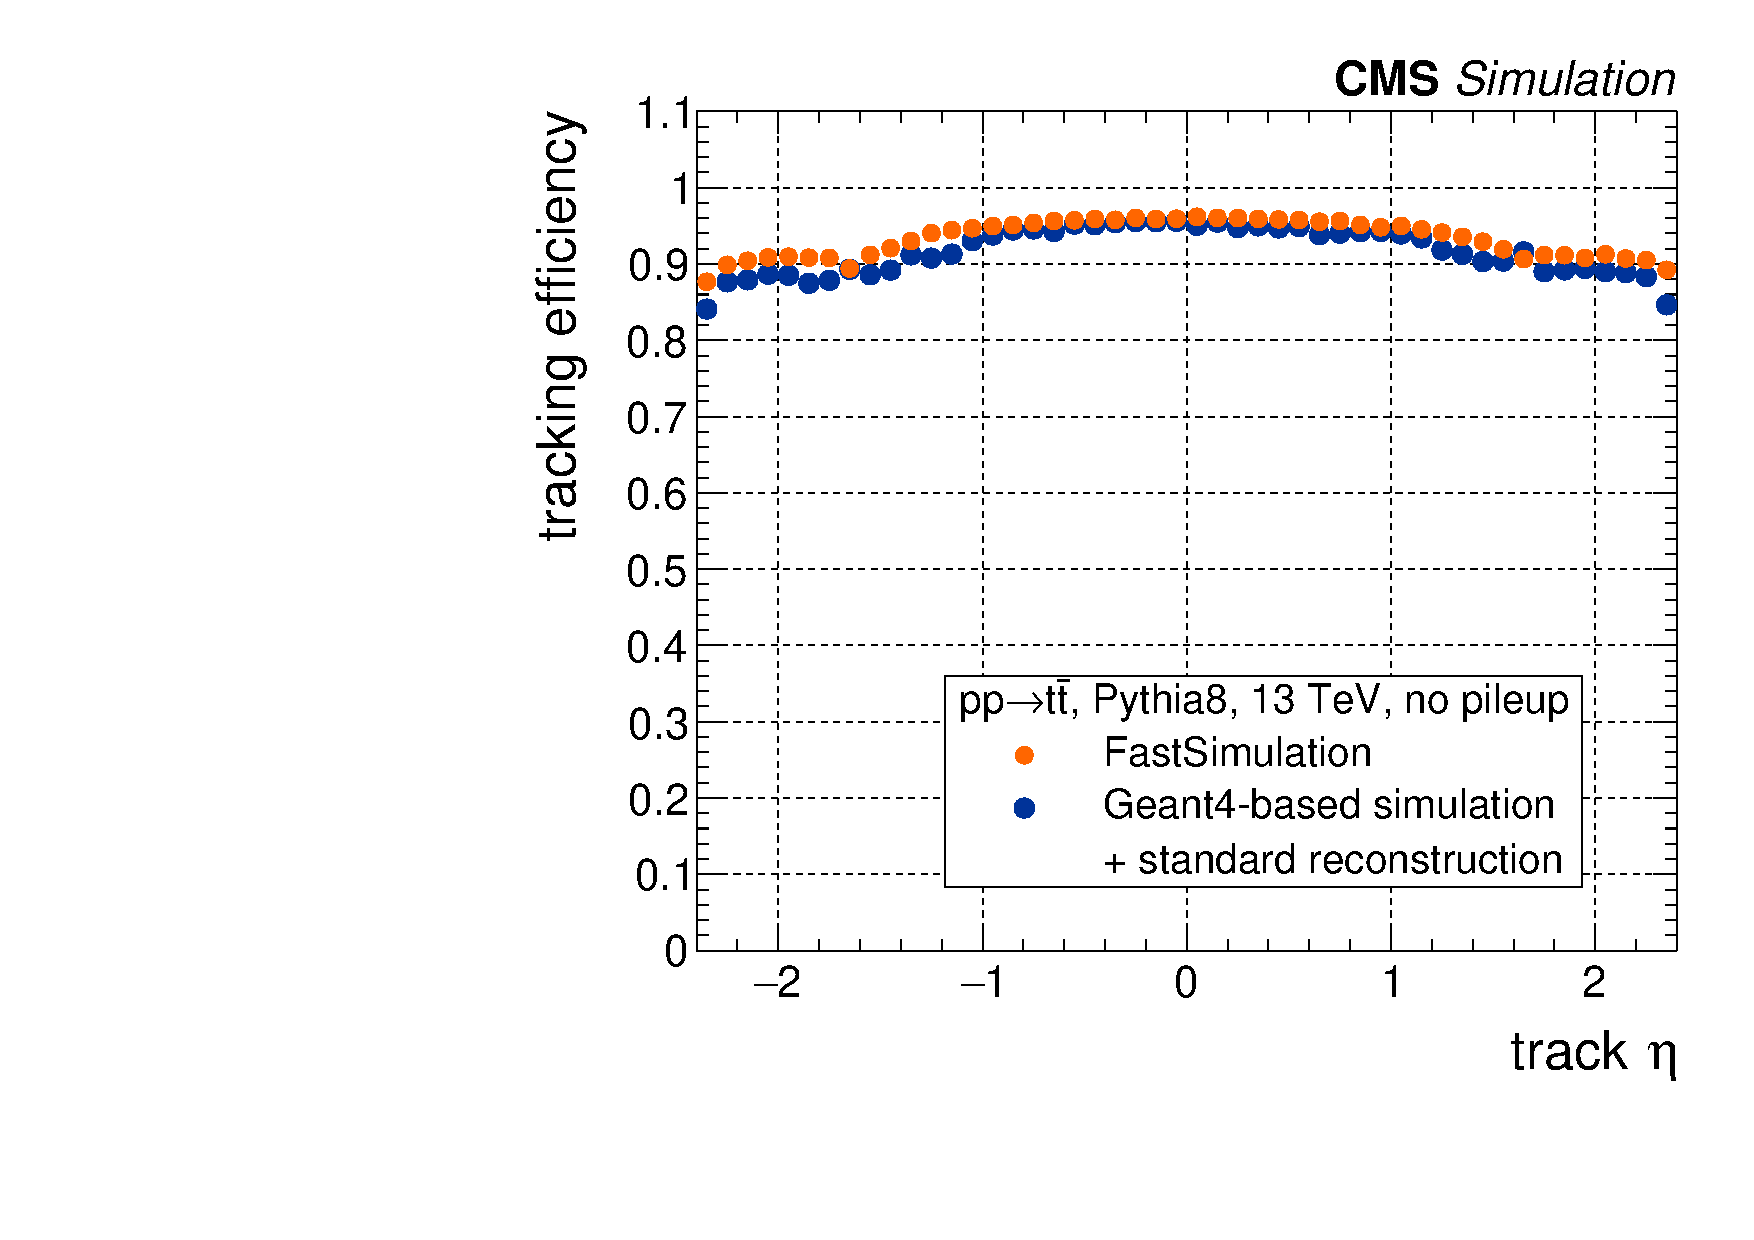
\includegraphics[width=0.48\textwidth]{figures/fastsim/eff_eta.pdf}}
}

A profile of the average CPU-time consumption per event within \FSIM is given in Fig.~\ref{fig:fsim-cpu} as a function of the average number of pileup interactions. Less than 10~s are required to simulated an event of top quark pair production for current pileup scenarios with $\approx30$ interactions on average. The presented emulation of tracking in this chapter is not amongst the top CPU consumers.

\myfigure{\label{fig:fsim-res-track}Comparison of the resolution of reconstructed tracks as a function of the transverse momentum measured in the simulation of top quark pair production at 13~TeV.}{
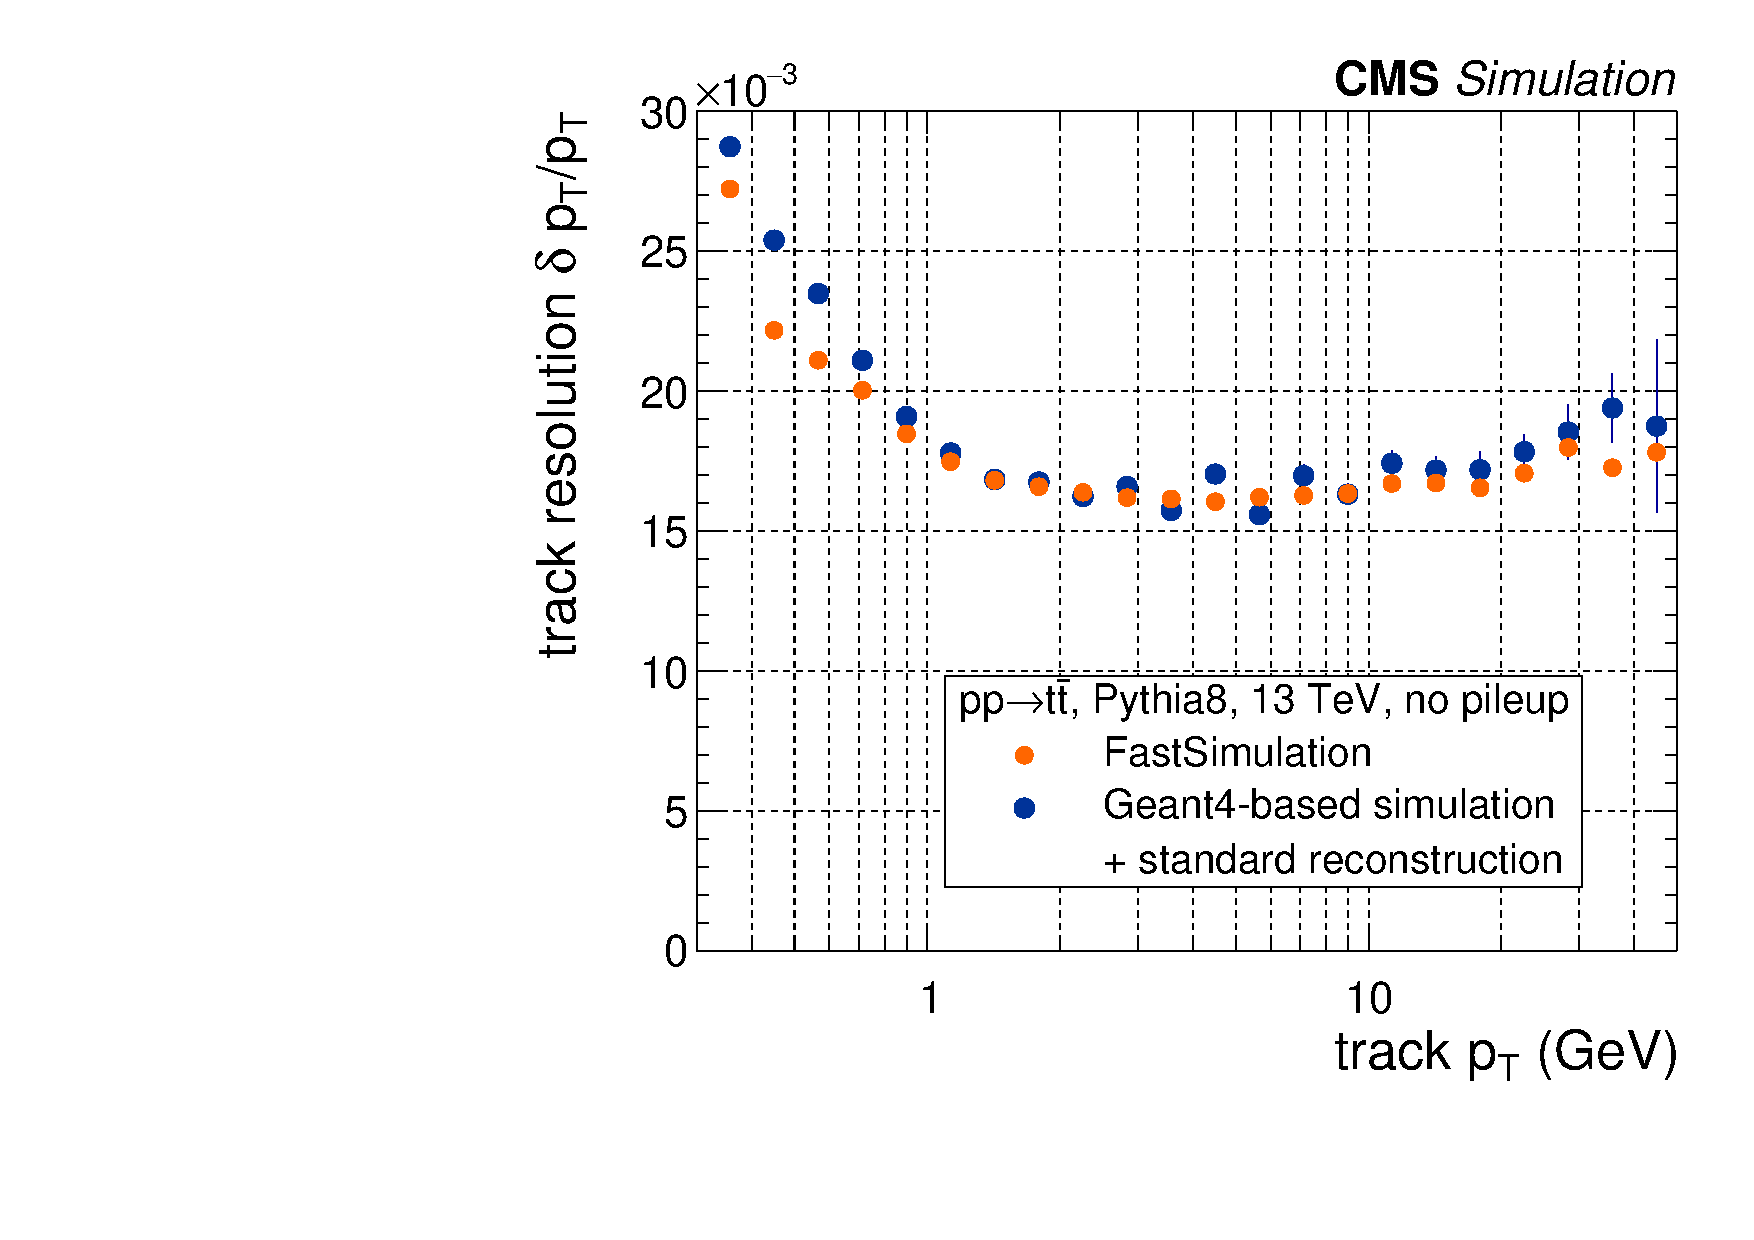
\includegraphics[width=0.48\textwidth]{figures/fastsim/res_pt.pdf}
}

\myfigure{\label{fig:fsim-cpu}Average CPU-time per event spent on the detector simulation and the reconstruction of analysis objects as a function of the average number of pileup interactions measured in the simulation of \ttbar production at 13~TeV using the \texttt{IgProf}~\cite{Eulisse:865673} profiler.}{
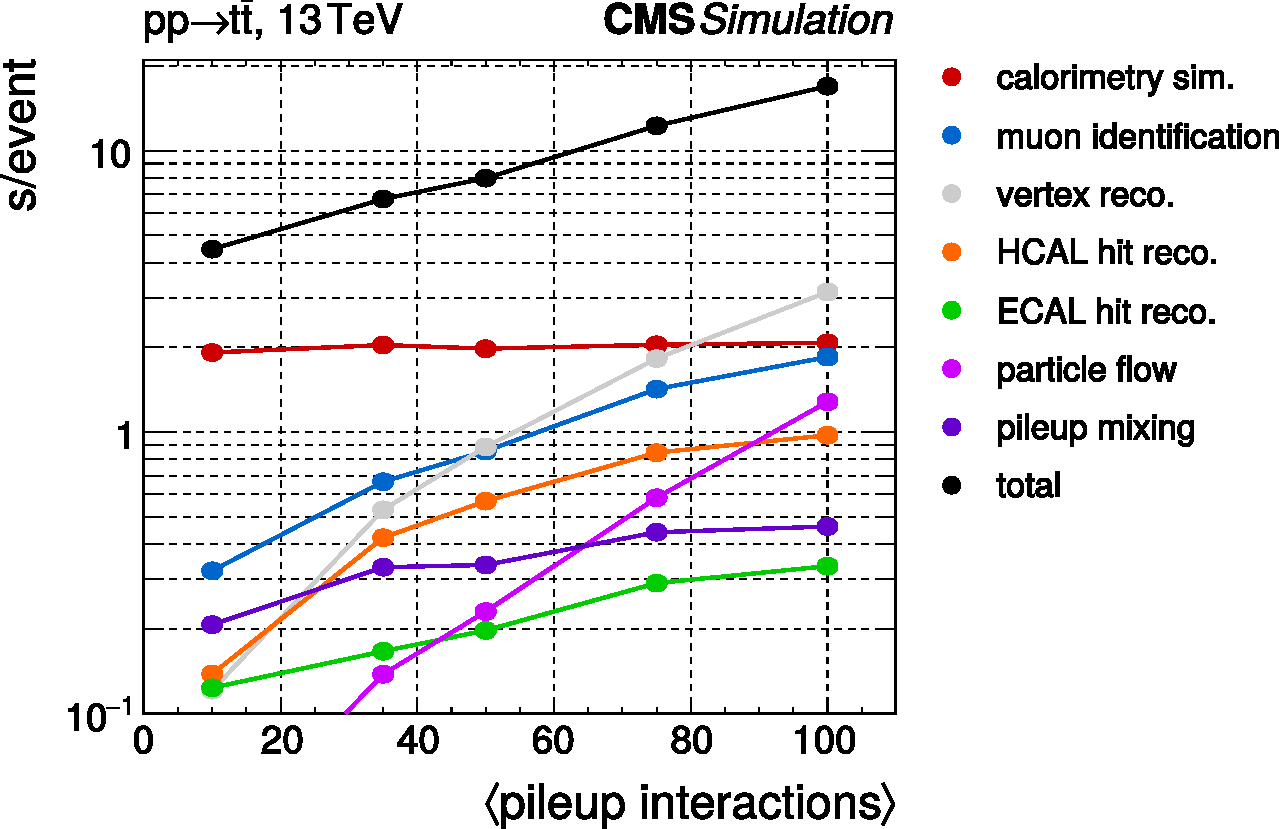
\includegraphics[width=0.65\textwidth]{figures/fastsim/cpu_profile.pdf}
}

%##############################################
\section{Conclusion}
%##############################################
\label{sec:fsim-conclusion}

The \gls{cms} \FSIM package provides a fast alternative to the standard simulation and reconstruction workflow for generation samples of simulated events. One of its major speedups is the usage of truth information in the track reconstruction. Recent developments in the framework led to further flexibility in the emulation of hit reconstruction and in the iterative tracking sequence. In the short term, these developments will enable the emulation of merged hits originating from close particle tracks. In the long term, the increased flexibility will allow to adapt the emulation of track reconstruction to the (planned) upgrades of the \gls{cms} detector.



